 \documentclass[pdftex,12pt, oneside]{article}

%\usepackage[paperwidth=8.5in, paperheight=13in]{geometry} % Folio
\usepackage[paperwidth=8.27in, paperheight=11.69in]{geometry} % A4

\usepackage{makeidx}         % allows index generation
\usepackage{graphicx}        % standard LaTeX graphics tool
                             % when including figure files
\usepackage[bottom]{footmisc}% places footnotes at page bottom
\usepackage[english]{babel}
\usepackage{enumerate}
\usepackage{paralist}
\usepackage{float}
\usepackage{gensymb}  
\usepackage{listings}
\usepackage{color}
\usepackage{mathtools} % atau \usepackage{amsmath}
\renewcommand{\baselinestretch}{1.5}

\newcommand{\HRule}{\rule{\linewidth}{0.5mm}}

\definecolor{codegreen}{rgb}{0,0.6,0}
\definecolor{codegray}{rgb}{0.5,0.5,0.5}
\definecolor{codepurple}{rgb}{0.58,0,0.82}
\definecolor{backcolor}{rgb}{0.95,0.95,0.92}

\lstdefinestyle{mystyle}{
  backgroundcolor=\color{backcolor},
  commentstyle=\color{codegreen},
  keywordstyle=\color{magenta},
  stringstyle=\color{codepurple},
  basicstyle=\footnotesize,
  breakatwhitespace=false,
  breaklines=true,
  captionpos=b,
  keepspaces=true,
  numbers=left,
  numbersep=5pt,
  showspaces=false,
  showstringspaces=false,
  showtabs=false,
  tabsize=2
}

\lstset{style=mystyle}


\begin{document}
\sloppy % biar section ga melebar melewati kertas

\begin{center}
{\large PETUNJUK OPERASIONAL SISTEM KOMPUTER - WS PBB}
\\[1cm]
XX Januari 2017\\
Priyanto Tamami, S.Kom.
\end{center}

%\frontmatter%%%%%%%%%%%%%%%%%%%%%%%%%%%%%%%%%%%%%%%%%%%%%%%%%%%%%%


%%%%%%%%%%%%%%%%%%%%%%%%%%%%%%%%%%%%%%%%%%%%%%%%%%%%%%%%%%%%%%%%%%%%%%

\section{PENDAHULUAN}

Sistem aplikasi ini digunakan untuk melakukan komunikasi dengan pihak Bank sebagai tempat pembayaran yang difungsikan untuk mencatatkan pembayaran Pajak Bumi dan Bangunan Perdesaan dan Perkotaan. 

Bentuk dari aplikasi ini hanya menyediakan \textit{Application Programming Interface} (API) untuk melakukan \textit{inquiry} data tagihan Pajak Bumi dan Bangunan Perdesaan dan Perkotaan, atau melakukan pencatatan pembayaran yang terjadi, atau melakukan \textit{reversal} bila terjadi kesalahan pencatatan pembayaran.

Karena implementasinya berbentuk REST API, maka jalur komunikasi yang digunakan sama dengan jalur komunikasi aplikasi \textit{web} pada umumnya, yaitu menggunakan \textit{port} 80.

\section{INSTALASI PROGRAM}

Instalasi program aplikasi \textit{web service} ini cukup mudah, karena hasil dari kompilasi kode ke bentuk program akan berbentuk sebuah \textit{file} berekstensi \texttt{war}, yang nantinya \textit{file} ini akan diunggah ke \textit{server} Tomcat untuk melayani \textit{browser} di masing-masing \textit{client}. Langkah instalasi yang dilakukan adalah sebagai berikut :

\begin{enumerate}[1.]
  \item Melakukan kompilasi kode yang menghasilkan \textit{file} berekstensi \texttt{war}.
  
  \item Melakukan unggah \textit{file} \texttt{war} ke \textit{server} Tomcat seperti pada gambar \ref{fig:deploy-war} berikut :
  
  \begin{figure}[H]
    \centering
    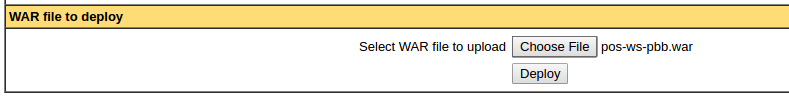
\includegraphics[width=1\textwidth]{./resources/001-deploy-war}
    \caption{\textit{Deploy File} \texttt{war}}
    \label{fig:deploy-war}
  \end{figure}
  
  \item Melakukan pengujian dengan melakukan akses ke \textit{server} menggunakan \textit{browser}, hasilnya akan terlihat seperti pada gambar \ref{fig:ws-worked} berikut :
  
  \begin{figure}[H]
    \centering
    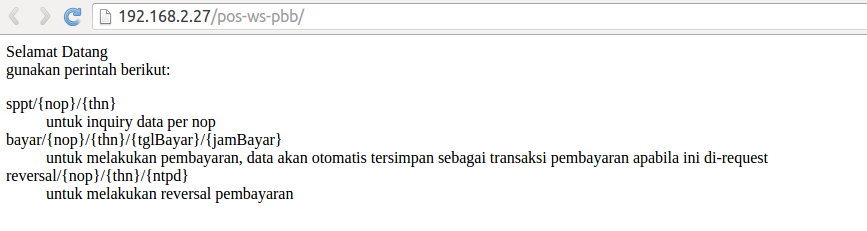
\includegraphics[width=1\textwidth]{./resources/002-ws-worked}
    \caption{Akses ke \textit{Web Service} Sudah Dapat Dilakukan}
    \label{fig:ws-worked}
  \end{figure}
  
  \item Selesai.
\end{enumerate}

\section{PROSEDUR OPERASI}

Sebagaimana terlihat pada gambar \ref{fig:ws-worked} bahwa ada 3 (tiga) layanan \textit{web service} yang diberikan yang dapat dilakukan dengan perintah melalui URL \textit{web} seperti berikut :

\begin{enumerate}[1.]
  \item \textit{Inquiry}
  \item Pencatatan Pembayaran
  \item \textit{Reversal} Pembayaran
\end{enumerate}

Dengan menggunakan \textit{web service} maka hanya ada 2 (dua) informasi dasar yang terjadi, yaitu berupa \textit{request} dan respon dalam dalam kata lain adalah \textit{input} dan \textit{output}. Penjelasan lebih rinci dari tiap layanan yang diberikan adalah sebagai berikut :

\subsection{\textit{Inquiry}}

Untuk \textit{inquiry} data tagihan, format \textit{request} yang dikirimkan adalah sebagai berikut :

\begin{lstlisting}
/sppt/{nop}/{thn}
\end{lstlisting}

Dengan keterangan sebagai berikut :

\begin{itemize}
  \item Parameter \texttt{\{nop\}} digantikan dengan Nomor Objek Pajak (NOP) untuk mengidentifikasi objek mana yang akan diambil informasinya.
  \item Parameter \texttt{\{thn\}} digantikan dengan Tahun Pajak untuk objek pajak yang akan diakses informasinya.
\end{itemize}

Hasil dari \textit{inquiry} di atas akan menghasilkan beberapa respon dari \textit{server}. Karena beberapa sebab, \textit{server} mungkin saja tidak dapat melakukan proses terhadap \textit{request} yang datang, sehingga diperlukan informasi yang cukup jelas sebagai informasi kepada \textit{client} bahwa \textit{request} yang dikirimkan berhasil atau gagal. 

Respon yang dikirimkan oleh \textit{server} akan menjadi bermacam-macam sesuai kondisinya, untuk memudahkan penjelasan, maka akan dibagi menjadi beberapa skenario berikut :

\begin{itemize}
  \item Skenario \textit{Inquiry} Yang Sukses
  \item Skenario \textit{Inquiry} Yang Gagal Karena Tahun Pajak Bukan Angka
  \item Skenario \textit{Inquiry} Yang Gagal Karena Data Tidak Ditemukan
  \item Skenario \textit{Inquiry} Yang Gagal Karena Kesalahan Server
\end{itemize}

Secara rinci akan dijelaskan sebagai berikut :

\subsubsection{Skenario \textit{Inquiry} Yang Sukses}

  Pada saat \textit{client} melakukan \textit{request inquiry} data ke \textit{server}, jika memang data tersebut ada pada basis data dan komunikasi berjalan sebagaimana mestinya, maka \textit{server} akan memberikan respon sebagai berikut :
  
  \begin{lstlisting}
{
  "code": 01,
  "message":"Data ditemukan",
  "sppt": {
    "nop":{nop},
    "thn":{thn},
    "nama":{nama wp},
    "alamatOp":{alamat op},
    "pokok":{pokok},
    "denda":{denda}
  }
}
  \end{lstlisting}
  
  Dengan keterangan sebagai berikut :
  
  \begin{itemize}
    \item \texttt{"code"}, berisi kode status respon dari \textit{server} yang menggambarkan suatu kondisi, jika kondisi \textit{inquiry} selesai di proses tanpa ada masalah, maka akan bernilai \texttt{01}.
    
    \item \texttt{"message"}, berisi pesan informasi dari kondisi respon \textit{server} yang telah terjadi, untuk menjelaskan kode status yang tertera pada bagian \texttt{"code"}.
    
    \item \texttt{"sppt"}, berisi informasi \textit{inquiry} yang di\textit{request} oleh \textit{client}.
    
    \item \texttt{\{nop\}}, nantinya akan terisi oleh Nomor Objek Pajak PBB-P2 yang di\textit{request} oleh \textit{client}.
    
    \item \texttt{\{thn\}}, nantinya akan terisi oleh tahun pajak untuk nomor objek pajak yang di\textit{request} oleh \textit{client}.
    
    \item \texttt{\{nama wp\}}, nantinya akan terisi oleh nama wajib pajak untuk nomor objek pajak dan tahun pajak yang diminta oleh \textit{client}.
    
    \item \texttt{\{alamat op\}}, nantinya akan terisi oleh alamat objek pajak untuk nomor objek pajak dan tahun pajak yang diminta oleh \textit{client}.
    
    \item \texttt{\{pokok\}}, nantinya akan terisi oleh besarnya pokok pajak terhutang.
    
    \item \texttt{\{denda\}}, nantinya akan terisi oleh besarnya denda administrasi yang harus 
  \end{itemize}

\subsubsection{Skenario \textit{Inquiry} Yang Gagal Karena Tahun Pajak Bukan Angka}

\subsubsection{Skenario \textit{Inquiry} Yang Gagal Karena Data Tidak Ditemukan}

\subsubsection{Skenario \textit{Inquiry} Yang Gagal Karena Kesalahan Server}

\subsection{Pencatatan Pembayaran}

\subsection{\textit{Reversal} Pembayaran}

\section{REFERENSI KODE}

\end{document}